To measure memory read latency we read the first byte of each cache line within a span of memory.  
We align the data to L1 cache lines.
We measure the time taken per read and then compute the mean and standard deviation of the time by span size.
As the span size increases, the depth of memory reached goes from L1 to L2 and finally to main memory.  
Larger spans would eventually reach to the secondary storage due to paging but very large spans would be needed and thus paging is measured in a later experiment.

The reading code follows this pseudo code pattern:
\begin{verbatim}
for(k = 0; k < 2^SPAN_SIZE; k+= PAGE_SIZE){
	x = data[k];
}
\end{verbatim}

If we had the whole L1/L2 cache to use, we'd expect to transition to L2 cache at N=14 and to main memory at N=17.
Since we likely don't have the whole cache and will likely have cache line collisions we'll proably move to deeper memory hierarchies a bit early.
Documentation shows that the L1 cache has a 3 cycle load-to-use delay.  
No documentation exists regarding the L2/Memory latency; however, an experiment similar to ours found latencies of 3 cycles for L1, 56 cycles for L2, and 116 cycles for memory\cite{sandmem}.
Instead of looping through an array of chars they constructed a linked list but otherwise performed a similar test.
Thus we expect similar results.

\begin{figure}[h]
\label{fig:exp_2_1}
\centering
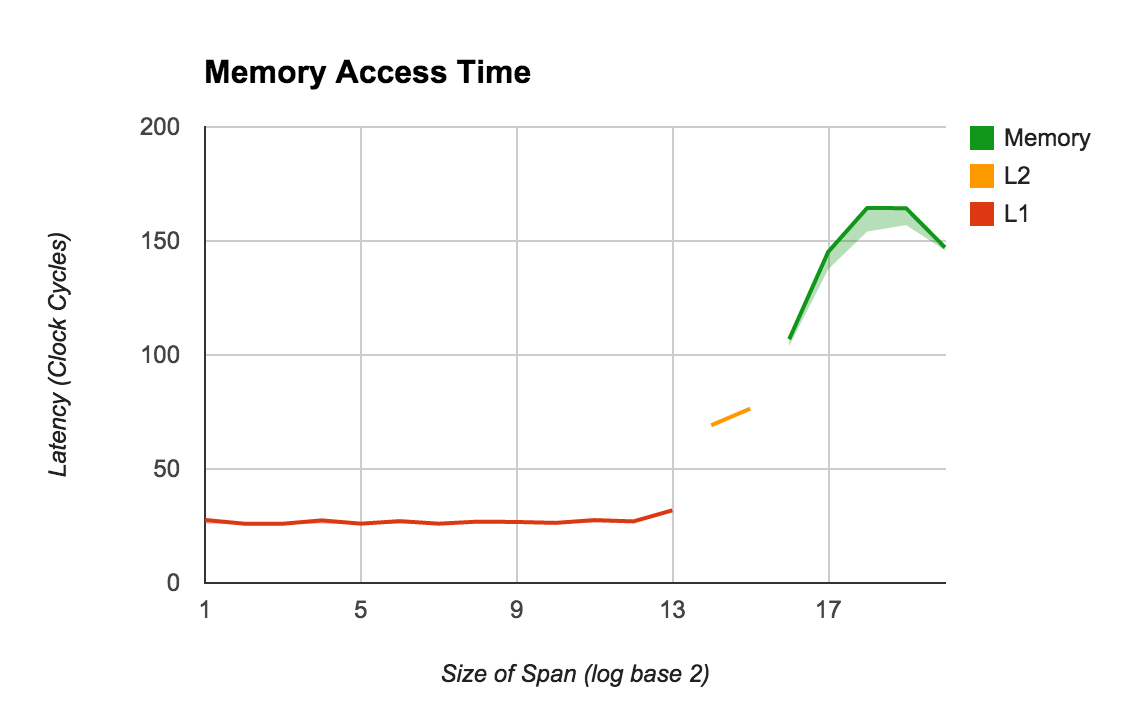
\includegraphics[scale=.5]{experiments/exp_2_1_fig.png}
\caption{Cycle count for memory read latency vs span size.  
Different memory regimes are labeled by color.  +/- 1 standard deviation highlighted by shading.}
\end{figure}

In Figure \ref{fig:exp_2_1} we see that the L1 cache latency averages 10 cycles, L2 averages 59 cycles, and main memory about 145 cycles, with a standard deviation of < 1 cycle for all levels. 
The L1 cache and Memory tests are slower than the cited experiment however the L2 is right on the mark.
It is possible that the linked list, which intrinsically does useful work (by pointing at the next location to work) vs our code which performs useful work outside of the timing cycle (by computing with and storing a new number into the array) results in additional overhead we don't expect.  

